\themaN
\graphicspath{{../Ch9_Fractions/Images/}}

\chapter{Fractions}
\label{C11}


%%%%%%%%%%%%%%%%%%%%%%%%%%%%%%%%%%%%%%%%%%
\begin{prerequis}[Connaissances et compétences abordées]
   \begin{itemize}
      \item Connaître diverses désignations des fractions : orales, écrites et décompositions additives et multiplicatives (ex : quatre tiers ; 4/3 ; 1/3 + 1/3 + 1/3 + 1/3 ; 4 x 1/3).
      \item Connaître et utiliser quelques fractions simples comme opérateur de partage en faisant le lien entre les formulations en langage courant et leur écriture mathématique.
      \item Repérer et placer des fractions sur une demi-droite graduée adaptée.
   \end{itemize}
\end{prerequis}

\vfill

\begin{debat}[Débat : les fractions, ces nombres rompus !] 
   C'est vers 3000 ans avant J.-C. que l'on trouve les premières représentations des fractions en Mésopotamie. Au {\small XII}\up{e} siècle, le mot {\bf fractiones} est traduit de l'arabe du mot {\it kasr}, qui veut dire {\it rompu}. En effet, à cette époque, les fractions sont considérées comme des nombres rompus : des nombres que l'on aurait cassé en plusieurs morceaux. Au {\small XIV}\up{e} siècle, le mathématicien {\it Nicole Oresme} utilise la notation des fractions avec la barre et définit les termes de numérateur et dénominateur.
   \begin{center}
      \textcolor{B1}{\fontsize{30}{30}\selectfont $\dfrac{a}{b} =a\div b =a\times\dfrac{1}{b}$}
   \end{center}
   \bigskip
   \begin{cadre}[B2][F4]
      \begin{center}
         Vidéo : \href{https://leblob.fr/fondamental/les-fractions}{\bf Les fractions}, site Internet {\it Le Blob, l'extra-média}.
      \end{center}
   \end{cadre}
\end{debat}

\vfill

\textcolor{PartieGeometrie}{\sffamily\bfseries Cahier de compétences} : chapitre 4, exercices 1 à 10 ; 31 à 45.


%%%%%%%%%%%%%%%%%%%%%%%%%%%%%%%%%%%%
%%%%%%%%%%%%%%%%%%%%%%%%%%%%%%%%%%%%
\activites

\begin{activite}[Des briques et des fractions]
   {\bf Objectifs :} utiliser des fractions pour exprimer une proportion ; utiliser le vocabulaire des fractions : moitié, tiers, quart\dots{} et leur correspondance rationnelle.
   \begin{QCM}
      \begin{minipage}{10cm}
         On considère la brique de Lego® classique ci-contre que l'on choisit comme unité. Caractériser les briques suivantes, par rapport à la brique unité. On pourra utiliser plusieurs formulations.
      \end{minipage}
      \hspace{2cm}
      \begin{minipage}{5cm}
         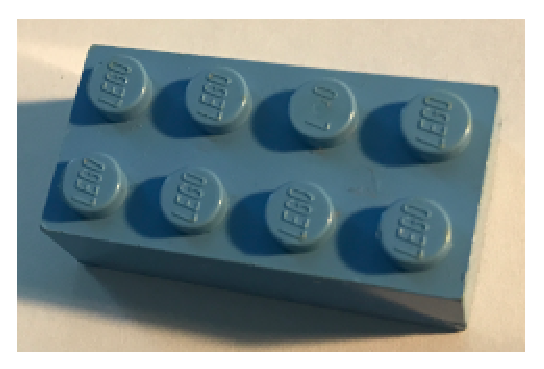
\includegraphics[width=3.5cm]{lego_4_2}
      \end{minipage}
      \partie[]
         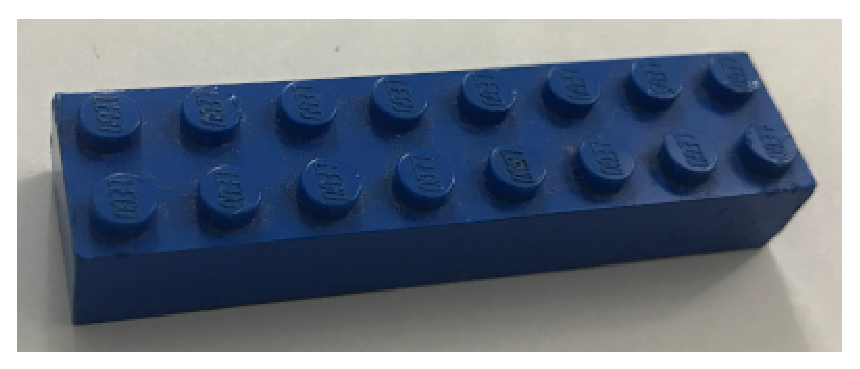
\includegraphics[height=2cm]{lego_8_2}
         \hspace{2.6cm}
         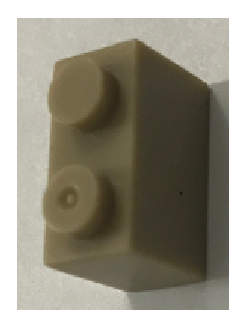
\includegraphics[height=2cm]{lego_2_1}
         \hspace{4.8cm}
         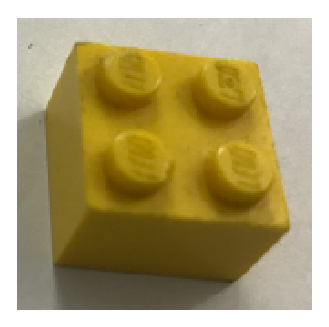
\includegraphics[height=2cm]{lego_2_2} \\ [2.5mm]
         \pf \hfill \pf \hfill \pf \\ [2.5mm]
         \pf \hfill \pf \hfill \pf \smallskip

      \partie[]
         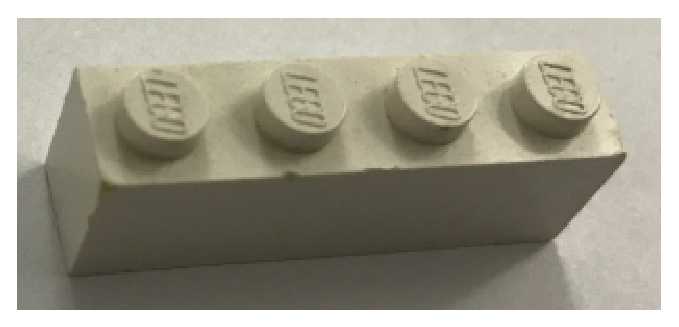
\includegraphics[height=2cm]{lego_4_1}
         \hspace{1.3cm}
         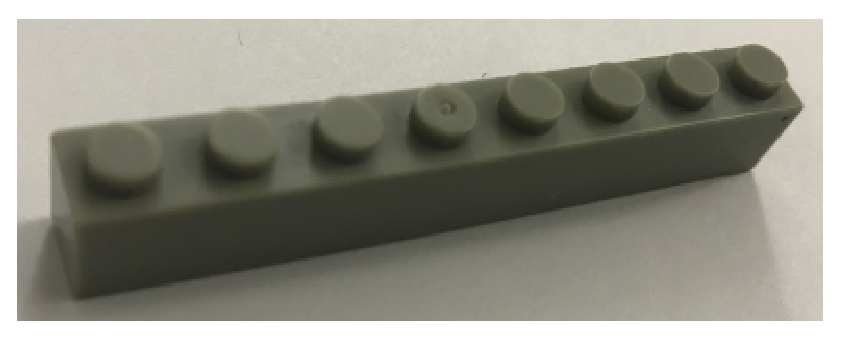
\includegraphics[height=2cm]{lego_8_1}
         \hspace{2.7cm}
         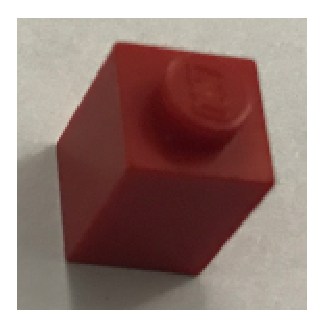
\includegraphics[height=2cm]{lego_1_1} \\ [2.5mm]
         \pf \hfill \pf \hfill \pf \\ [2.5mm]
         \pf \hfill \pf \hfill \pf \smallskip
         
      \partie[]
         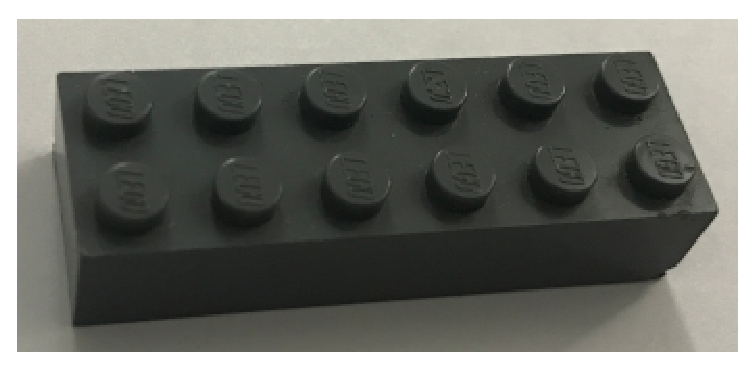
\includegraphics[height=2cm]{lego_6_2}
         \hspace{2.8cm}
         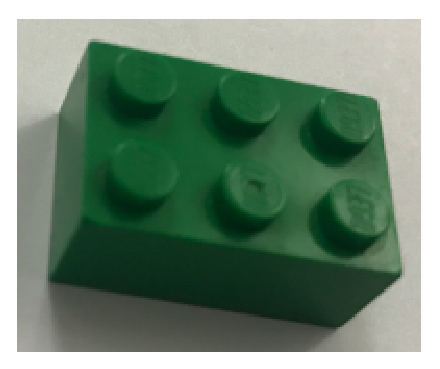
\includegraphics[height=2cm]{lego_3_2}
         \hspace{2.5cm}
         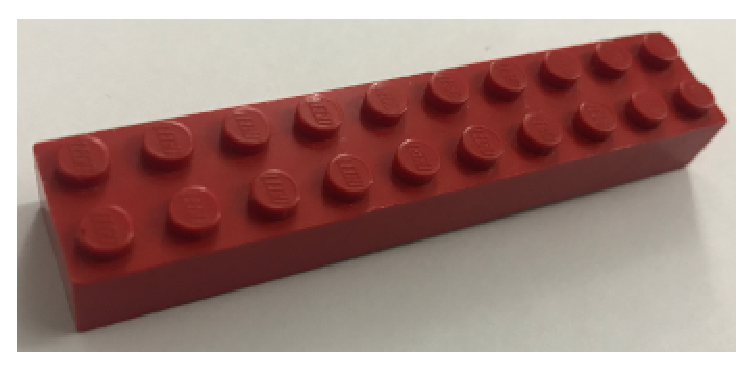
\includegraphics[height=2cm]{lego_10_2} \\ [2.5mm]
         \pf \hfill \pf \hfill \pf \\ [2.5mm]
         \pf \hfill \pf \hfill \pf \smallskip
      
      \partie[]
         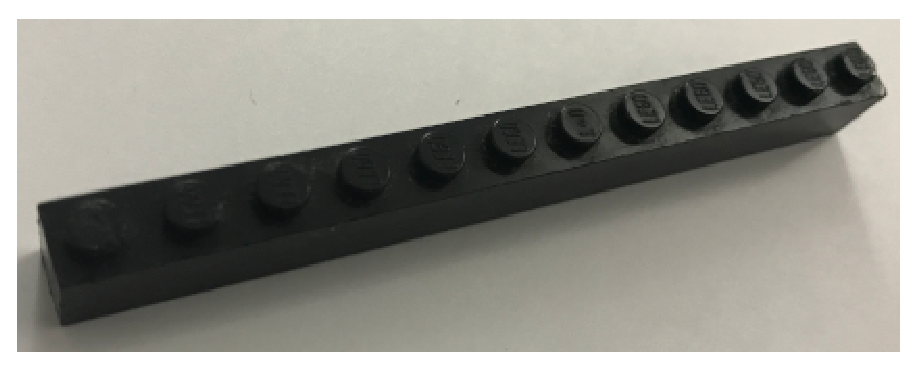
\includegraphics[height=2cm]{lego_12_1}
         \hspace{0.5cm}
         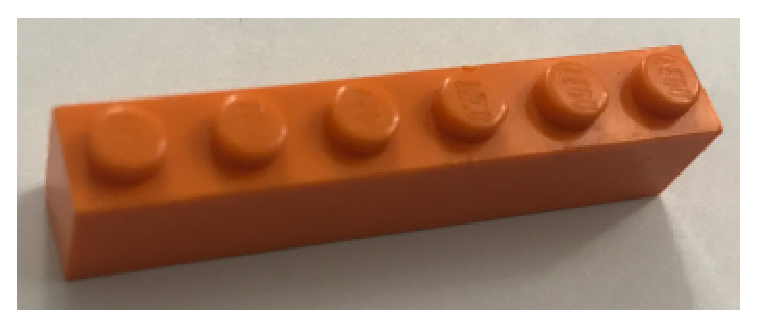
\includegraphics[height=2cm]{lego_6_1}
         \hspace{2cm}
         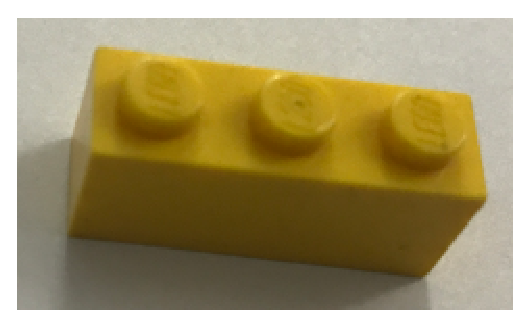
\includegraphics[height=2cm]{lego_3_1} \\ [2.5mm]
         \pf \hfill \pf \hfill \pf \\ [2.5mm]
         \pf \hfill \pf \hfill \pf \medskip
   \end{QCM}
\end{activite}
   

%%%%%%%%%%%%%%%%%%%%%%%%%%%%%%%%%%%%
%%%%%%%%%%%%%%%%%%%%%%%%%%%%%%%%%%%%
\cours 

%%%%%%%%%%%%%%%%%%%%%%%%%%
\section{Différentes manière de penser les fractions}

\begin{definition}
   Une \textbf{fraction} indique quelle partie d'un tout on doit prendre, elle peut représenter un {\bf partage}, une {\bf proportion}.
\end{definition}

\bigskip

On partage une pizza en quatre parts égales.

\begin{center}
   {\small
   \begin{tabular}{C{3}C{3}C{3.5}C{4}}
      \begin{pspicture}(-1,-1.1)(1,1.1)
         \rput(0,0){
\includegraphics[width=2cm]{pizza}}
         \pscircle(0,0){1}
         \psset{linecolor=white,fillstyle=solid,fillcolor=white}
         \pswedge(0,0){0.98}{90}{0}
         \psset{linecolor=black}
         \psline(-1,0)(1,0)
         \psline(0,-1)(0,1)  
      \end{pspicture}
      &
      \begin{pspicture}(-1,-1.1)(1,1.1)
         \rput(0,0){
\includegraphics[width=2cm]{pizza}}
         \pscircle(0,0){1}
        \psset{linecolor=white,fillstyle=solid,fillcolor=white}
         \pswedge(0,0){0.98}{180}{0}
         \psline[linewidth=0.7mm](0,0)(0,1) 
         \psset{linecolor=black}
         \psline(-1,0)(1,0)
         \psline(0,-1)(0,0)  
      \end{pspicture}
      &
      \begin{pspicture}(-1,-1.1)(1,1.1)
         \rput(0,0){
\includegraphics[width=2cm]{pizza}}
         \pscircle(0,0){1}
         \psset{linecolor=white,fillstyle=solid,fillcolor=white}
         \pswedge(0,0){0.98}{-90}{0}
         \psline[linewidth=0.7mm](-1,0)(1,0)
         \psline[linewidth=0.7mm](0,0)(0,1)
      \end{pspicture}
      &
      \begin{pspicture}(-1,-1.1)(1,1.1)
         \rput(0,0){
\includegraphics[width=2cm]{pizza}}
        \pscircle(0,0){1}
         \psset{linewidth=0.7mm,linecolor=white}
         \psline(-1,0)(1,0)
         \psline(0,-1)(0,1) 
      \end{pspicture} \\
      {\bf une} part & \textbf{deux} parts & \textbf{trois} parts & \textbf{quatre} parts \\   
      un {\bf quart} de pizza & deux {\bf quarts} de pizza & trois {\bf quarts} de pizza & quatre {\bf quarts} de pizza \\ [2mm]
      $\dfrac14$ & $\dfrac24 =\dfrac14+\dfrac14 =2\times\dfrac14$ & $\dfrac34 =\dfrac14+\dfrac14+\dfrac14 =3\times\dfrac14$ & $\dfrac44 =\dfrac14+\dfrac14+\dfrac14+\dfrac14 =4\times\dfrac14$ \\ 
   \end{tabular}}
\end{center}

\smallskip

\begin{minipage}{10cm}
   Et si on mangeait plus d'une pizza ? \\
   Dans ce cas, on obtient une fraction supérieure à 1. \\
   On a pris {\bf sept} parts de pizza, soit $\dfrac74$ de pizza. \\
   On peut aussi dire {\bf une} pizza et {\bf trois} quarts de pizza, soit $1+\dfrac34$.
\end{minipage}
\qquad
\begin{minipage}{6cm}
   \begin{pspicture}(-1,-1.2)(1,1.2)
      \rput(0,0){
\includegraphics[width=2cm]{pizza}}
      \pscircle(0,0){1}
      \psset{linewidth=0.7mm,linecolor=white}
      \psline(-1,0)(1,0)
      \psline(0,-1)(0,1) 
   \end{pspicture}
   \qquad 
   \begin{pspicture}(-1,-1.2)(1,1.2)
      \rput(0,0){
\includegraphics[width=2cm]{pizza}}
      \pscircle(0,0){1}
      \psset{linecolor=white,fillstyle=solid,fillcolor=white}
      \pswedge(0,0){0.98}{-90}{0}
      \psline[linewidth=0.7mm](-1,0)(1,0)
      \psline[linewidth=0.7mm](0,0)(0,1)
   \end{pspicture}
\end{minipage}


\begin{definition}
   Soit $a$ et $b$ deux nombres ($b\neq0$). Le {\bf quotient} $\dfrac{a}{b}$ est le nombre qui, multiplié par $b$, donne $a$. \\
   Ce quotient écrit sous forme d'une fraction est le résultat d'une division : $\dfrac{a}{b} =a\div b$.
\end{definition}

\begin{exemple}
   La fraction $\dfrac73$ peut être interprétée comme :
   \correction
   \ \\ [-10mm]
   \begin{itemize}
      \item $7\div3$, dont une valeur approchée est 2,33 ;
      \item sept tiers ;
      \item le nombre qui, multiplié par $3$, donne $7$.
   \end{itemize}
\end{exemple}

\begin{remarque} 
   quand on partage une quantité en 
   \begin{itemize}
      \item  \textbf{deux} parts égales, on obtient des \textbf{demis}, le \textbf{double} d'un demi fait un.
      \item \textbf{trois} parts égales, on obtient des \textbf{tiers}, le \textbf{triple} d'un tiers fait un.
      \item \textbf{quatre} parts égales, on obtient des \textbf{quarts}, le \textbf{quadruple} d'un quart fait un.
   \end{itemize}
\end{remarque}


%%%%%%%%%%%%%%%%%%%%%%%%%%%%%%%%
\section{Repérage sur une demi-droite graduée}

Comme tous les autres nombres, on peut placer les fractions sur une droite graduée.

\begin{exemple*1}
   Si on partage l'unité d'une droite graduée en quatre, on peut placer des \og quarts \fg.
   \begin{center}
   \begin{pspicture}(0,0.2)(13,0.7)
      \psaxes[dx=1,yAxis=false,labels=none]{->}(0,0)(13,0)
      \rput(0,-0.3){0}
      \rput(4,-0.3){1}
      \rput(8,-0.3){2}
      \rput(12,-0.3){3}
      \uput[u](0,.1){$\frac04$}
      \uput[u](1,.1){$\frac14$}
      \uput[u](2,.1){$\frac24$}
      \uput[u](3,.1){$\frac34$}
      \uput[u](4,.1){$\frac44$}
      \uput[u](5,.1){$\frac54$}
      \uput[u](6,.1){$\frac64$}
      \uput[u](7,.1){$\frac74$}
      \uput[u](8,.1){$\frac84$}
      \uput[u](9,.1){$\frac94$}
      \uput[u](10,.1){$\frac{10}{4}$}
      \uput[u](11,.1){$\frac{11}{4}$}
      \uput[u](12,.1){$\frac{12}{4}$}
   \end{pspicture}
   \end{center}
\end{exemple*1}


%%%%%%%%%%%%%%%%%%%%%%%%%%%%%%%%%%%%%%%%%%
\exercicesbase

\begin{colonne*exercice}

\serie{Fractions}

\begin{exercice} %1
   Ecrire la fraction qui représente la partie colorée de chaque figure ci-dessous :
   \begin{center}
      \psset{unit=0.65}
      \begin{pspicture}(-1,-1.5)(2,1)
         \psframe[fillstyle=solid,fillcolor=A2](0,0)(-1,-1)
         \psframe(-1,-1)(1,1)
         \psline(-1,0)(1,0)
         \psline(0,-1)(0,1)
         \rput(-1.4,0){$a$}
      \end{pspicture}
      \begin{pspicture}(-1,-1.5)(2,1)
         \pspolygon[fillstyle=solid,fillcolor=A2](0,0)(0,-1)(1,-1)(1,1)(1,1)(-1,1)(-1,0)
         \psframe(-1,-1)(1,1)
         \psline(-1,0)(1,0)
         \psline(0,-1)(0,1)
         \rput(-1.4,0){$b$}
      \end{pspicture}
      \begin{pspicture}(-1,-1.5)(2,1)
         \psframe[fillstyle=solid,fillcolor=A2](-1,-1)(1,0)
         \psframe(-1,-1)(1,1)
         \psline(-1,0)(1,0)
         \psline(0,-1)(0,1)
         \rput(-1.4,0){$c$}
      \end{pspicture}
      \begin{pspicture}(-1,-1.5)(1,1)
         \psframe[fillstyle=solid,fillcolor=A2](-1,-1)(1,1)
         \psline(-1,0)(1,0)
         \psline(0,-1)(0,1)
         \rput(-1.4,0){$d$}
      \end{pspicture}
      
      \begin{pspicture}(-1,-1.5)(2,1)
         \pswedge[fillstyle=solid,fillcolor=B2](0,0){1}{30}{-30}
         \pscircle(0,0){1}
         \multido{\n=0+30}{12}{\psline(0,0)(1;\n)}
         \rput(-1.4,0){$e$}
      \end{pspicture}
      \begin{pspicture}(-1,-1.5)(2,1)
         \pswedge[fillstyle=solid,fillcolor=B2](0,0){1}{90}{180}
         \pscircle(0,0){1}
         \multido{\n=0+30}{12}{\psline(0,0)(1;\n)}
         \rput(-1.4,0){$f$}
      \end{pspicture}
      \begin{pspicture}(-1,-1.5)(2,1)
         \pswedge[fillstyle=solid,fillcolor=B2](0,0){1}{-120}{-60}
         \pscircle(0,0){1}
         \multido{\n=0+30}{12}{\psline(0,0)(1;\n)}
         \rput(-1.4,0){$g$}
      \end{pspicture}
      \begin{pspicture}(-1,-1.5)(1,1)
         \pswedge[fillstyle=solid,fillcolor=B2](0,0){1}{60}{-120}
         \pscircle(0,0){1}
         \multido{\n=0+30}{12}{\psline(0,0)(1;\n)}
         \rput(-1.4,0){$h$}
      \end{pspicture}
      
      \begin{pspicture}(-1,-1.2)(2,1.3)
         \pspolygon[fillstyle=solid,fillcolor=H1](1.2;210)(0,-0.6)(1.2;90)
         \pspolygon(1.2;-30)(1.2;90)(1.2;210)
         \psline(0.6;150)(1.2;-30)
         \psline(0.6;30)(1.2;210)
         \psline(0,-0.6)(0,1.2)
         \rput(-1.4,0.25){$i$}
      \end{pspicture}
      \begin{pspicture}(-1,-1.2)(2,1.3)
         \pspolygon[fillstyle=solid,fillcolor=H1](0,0)(1.2;-30)(0,-0.6)
         \pspolygon[fillstyle=solid,fillcolor=H1](0,0)(1.2;210)(0.6;150)
         \pspolygon[fillstyle=solid,fillcolor=H1](0,0)(1.2;90)(0.6;30)
         \pspolygon(1.2;-30)(1.2;90)(1.2;210)
         \psline(0.6;150)(1.2;-30)
         \psline(0.6;30)(1.2;210)
         \psline(0,-0.6)(0,1.2)
         \rput(-1.4,0.25){$j$}
      \end{pspicture}
      \begin{pspicture}(-1,-1.2)(2,1.3)
         \pspolygon[fillstyle=solid,fillcolor=H1](0,0)(0.6;30)(1.2;90)(0.6;150)
         \pspolygon(1.2;-30)(1.2;90)(1.2;210)
         \psline(0.6;150)(1.2;-30)
         \psline(0.6;30)(1.2;210)
         \psline(0,-0.6)(0,1.2)
         \rput(-1.4,0.25){$k$}
      \end{pspicture}
      \begin{pspicture}(-1,-1.2)(1,1.3)
         \pspolygon[fillstyle=solid,fillcolor=H1](0,0)(0.6;30)(1.2;90)(1.2;210)(1.2;-30)
         \pspolygon(1.2;-30)(1.2;90)(1.2;210)
         \psline(0.6;150)(1.2;-30)
         \psline(0.6;30)(1.2;210)
         \psline(0,-0.6)(0,1.2)
         \rput(-1.4,0.25){$l$}
      \end{pspicture}
      
      \begin{pspicture}(-1,-1.5)(2,1)
         \psgrid[subgriddiv=2,subgridcolor=black,subgridwidth=0.8pt,gridlabels=0](-1,-1)(1,1)
         \psframe[fillstyle=solid,fillcolor=J1](-1,0)(0,1)
         \rput(-1.4,0){$m$}
      \end{pspicture}
      \begin{pspicture}(-1,-1.5)(2,1)
         \psgrid[subgriddiv=2,subgridcolor=black,subgridwidth=0.8pt,gridlabels=0](-1,-1)(1,1)
         \psframe[fillstyle=solid,fillcolor=J1](-1,0)(0,1)
         \psframe[fillstyle=solid,fillcolor=J1](0,0.5)(0.5,0)
         \psframe[fillstyle=solid,fillcolor=J1](-1,-0.5)(-0.5,0)
         \rput(-1.4,0){$n$}
      \end{pspicture}
      \begin{pspicture}(-1,-1.5)(2,1)
         \psgrid[subgriddiv=2,subgridcolor=black,subgridwidth=0.8pt,gridlabels=0](-1,-1)(1,1)
         \psframe[fillstyle=solid,fillcolor=J1](-1,-1)(1,0)
         \psframe[fillstyle=solid,fillcolor=J1](-1,0)(0,1)
         \psframe[fillstyle=solid,fillcolor=J1](0,0)(0.5,0.5)
         \rput(-1.4,0){$p$}
      \end{pspicture}
      \begin{pspicture}(-1,-1.5)(1,1)
         \psgrid[subgriddiv=2,subgridcolor=black,subgridwidth=0.8pt,gridlabels=0](-1,-1)(1,1)
         \psframe[fillstyle=solid,fillcolor=J1](-1,-1)(0.5,0)
         \psframe[fillstyle=solid,fillcolor=J1](-1,0)(-0.5,1)
         \psframe[fillstyle=solid,fillcolor=J1](0.5,-0.5)(1,0)
         \rput(-1.4,0){$q$}
      \end{pspicture}
      
   \end{center}
\end{exercice}
   
\begin{exercice} %2
   Dans chaque figure ci-dessous, colorier selon la fraction donnée.
   \begin{center}
   \small
      \psset{unit=0.9}
      \begin{pspicture}(-1,-1.3)(1.7,1)
         \psframe(-1,-1)(1,1)
         \rput(1.25,0){$\dfrac13$}
      \end{pspicture}
      \begin{pspicture}(-1,-1.3)(1.7,1)
         \psframe(-1,-1)(1,1)
         \rput(1.25,0){$\dfrac34$}
      \end{pspicture}
      \begin{pspicture}(-1,-1.3)(1.5,1)
         \psframe(-1,-1)(1,1)
         \rput(1.25,0){$\dfrac58$}
      \end{pspicture}
      
      \begin{pspicture}(-1,-1.3)(1.7,1)
         \pscircle(0,0){1}
         \rput(1.25,0){$\dfrac13$}
      \end{pspicture}
      \begin{pspicture}(-1,-1.3)(1.7,1)
         \pscircle(0,0){1}
         \rput(1.25,0){$\dfrac34$}
      \end{pspicture}
      \begin{pspicture}(-1,-1.3)(1.5,1)
         \pscircle(0,0){1}
         \rput(1.25,0){$\dfrac58$}
      \end{pspicture}
      
      \begin{pspicture}(-1,-1.3)(1.7,1)
         \pspolygon(1;30)(1;90)(1;150)(1;210)(1;270)(1;330)
         \rput(1.25,0){$\dfrac13$}
      \end{pspicture}
      \begin{pspicture}(-1,-1.3)(1.7,1)
         \pspolygon(1;30)(1;90)(1;150)(1;210)(1;270)(1;330)
         \rput(1.25,0){$\dfrac34$}
      \end{pspicture}
      \begin{pspicture}(-1,-1.3)(1.5,1)
         \pspolygon(1;30)(1;90)(1;150)(1;210)(1;270)(1;330)
         \rput(1.25,0){$\dfrac56$}
      \end{pspicture}

      \begin{pspicture}(-1,-1.3)(1.7,1)
         \pspolygon(-1,-0.33)(-1,0.33)(-0.33,0.33)(-0.33,1)(0.33,1)(0.33,0.33)(1,0.33)(1,-0.33)(0.33,-0.33)(0.33,-1)(-0.33,-1)(-0.33,-0.33)
         \rput(1.25,0){$\dfrac14$}
      \end{pspicture}
      \begin{pspicture}(-1,-1.3)(1.7,1)
         \pspolygon(-1,-0.33)(-1,0.33)(-0.33,0.33)(-0.33,1)(0.33,1)(0.33,0.33)(1,0.33)(1,-0.33)(0.33,-0.33)(0.33,-1)(-0.33,-1)(-0.33,-0.33)
         \rput(1.25,0){$\dfrac38$}
      \end{pspicture}
      \begin{pspicture}(-1,-1.3)(1.5,1)
         \pspolygon(-1,-0.33)(-1,0.33)(-0.33,0.33)(-0.33,1)(0.33,1)(0.33,0.33)(1,0.33)(1,-0.33)(0.33,-0.33)(0.33,-1)(-0.33,-1)(-0.33,-0.33)
         \rput(1.25,0){$\dfrac25$}
      \end{pspicture}
   \end{center}
\end{exercice}

\begin{exercice} %3
   Écrire chaque désignation sous la forme d'une fraction, d'une somme de fractions et d'un produit comme dans l'exemple : $\dfrac24 =\dfrac14+\dfrac14 =2\times\dfrac14$. \smallskip
   \begin{colenumerate}{2}
      \item trois cinquièmes
      \item quatre tiers
      \item cinq septièmes
      \item six centièmes
   \end{colenumerate}
\end{exercice}

\begin{exercice} %4
   Sur la figure suivante, on a représenté un réseau de droites parallèles et équidistantes ainsi qu'un segment de longueur $u$ à trois reprises. À l'aide du compas, tracer sur le cahier les segments de longueur suivante :
   \smallskip
   \begin{colenumerate}{6}
      \item $\dfrac16u$
      \item $\dfrac15u$
      \item $\dfrac13u$
      \item $\dfrac56u$
      \item $\dfrac23u$
      \item $\dfrac35u$
   \end{colenumerate}
   \medskip
   \psset{xunit=0.7,yunit=0.3}
   \begin{pspicture*}(0,0)(11,8)
      \multido{\n=-3+1,\i=1+1}{14}{\psline[linecolor=gray](\n,0)(\i,8)}
       \psline[linewidth=0.5mm]{|-|}(0.5,3)(5.8,7.6)
      \psline[linewidth=0.5mm]{|-|}(2,2)(8.4,4.8)
      \psline[linewidth=0.5mm]{|-|}(3.5,1)(10.3,2.6)
      \rput(10.6,2.6){$u$}
      \rput(8.7,4.8){$u$}
      \rput(6.2,7.6){$u$}
   \end{pspicture*}
\end{exercice}

\begin{exercice} %5
   Compléter les phrases ci-dessous avec des mots.
   \begin{enumerate}
      \item 6 mois représentent \pf année.
      \item 4 mois représentent \pf année.
      \item 30 minutes représentent \pf heure.
      \item 45 minutes représentent \pf heure.
   \end{enumerate}
\end{exercice}

\medskip

\begin{exercice} %6
   Par quel nombre faut-il :
   \begin{enumerate}
      \item multiplier 5 pour obtenir 3 ?
      \item multiplier 19 pour obtenir 97 ?
      \item multiplier 12 pour obtenir 11 ?
   \end{enumerate}
\end{exercice}

%%%%%%%%%%%%%
\serie{Repérage}

\begin{exercice} %7
   Écrire l'abscisse de chaque point à l'aide d'une ou plusieurs fractions.
   {\small
   \begin{enumerate}
      \item \begin{pspicture}(0,0)(8,0.7)
                  \psset{xunit=5}
                  \psaxes[yAxis=false,subticks=10,subtickwidth=0.7pt]{->}(0,0)(1.5,0)
                  \pstGeonode[PosAngle=90](0.3,0){A}(0.8,0){C}(1.1,0){D}(1.3,0){B}
               \end{pspicture}
      \item \begin{pspicture}(0,0)(8,1.2)
                  \psset{xunit=3}
                  \psaxes[yAxis=false,subticks=5,subtickwidth=0.7pt]{->}(0,0)(2.5,0)
                  \pstGeonode[PosAngle=90](0.2,0){F}(0.6,0){E}(2.2,0){G}(1.8,0){H}
               \end{pspicture}
      \item \begin{pspicture}(0,0)(8,1.2)
                  \psset{xunit=4}
                  \psaxes[yAxis=false,subticks=8,subtickwidth=0.7pt]{->}(0,0)(1.9,0)
                  \pstGeonode[PosAngle=90](0.25,0){J}(1.125,0){K}(1.5,0){L}(0.625,0){M}
               \end{pspicture}
      \item \begin{pspicture}(0,-0.5)(8,1.2)
                  \psset{xunit=3}
                  \psaxes[yAxis=false,subticks=12,subtickwidth=0.7pt]{->}(0,0)(2.5,0)
                  \pstGeonode[PosAngle=90](0.25,0){P}(1.67,0){Q}(1,0){N}(2.08,0){R}
               \end{pspicture}
   \end{enumerate}}
\end{exercice}

\medskip

\begin{exercice} %8
   Placer les points donnés sur chaque demi-droite.
   \smallskip
   {\small
   \begin{enumerate}
      \item $S\left(\dfrac56\right)$ \; ; \; $T\left(\dfrac26\right)$ \; ; \; $U\left(\dfrac96\right)$ \; et \; $V\left(\dfrac66\right)$. \\
        \begin{pspicture}(0,-0.5)(8,0.5)
           \psset{xunit=4}
           \psaxes[yAxis=false,subticks=6,subtickwidth=0.7pt]{->}(0,0)(1.9,0)
        \end{pspicture}
        \item $W\left(\dfrac{7}{15}\right)$ \; ; \; $X\left(\dfrac{17}{15}\right)$ \; ; \; $Y\left(\dfrac{3}{15}\right)$ \; et \; $Z\left(\dfrac{10}{15}\right)$. \\
        \begin{pspicture}(0,-0.5)(8,0.5)
           \psset{xunit=5}
           \psaxes[yAxis=false,subticks=15,subtickwidth=0.7pt]{->}(0,0)(1.4,0)
        \end{pspicture} 
   \end{enumerate}}
\end{exercice}

\end{colonne*exercice}


%%%%%%%%%%%%%%%%%%%%%%%%%%%%%%%
%%%%%%%%%%%%%%%%%%%%%%%%%%%%%%%
\Recreation
   \enigme[L'atelier des potions]
      \partie[présentation du jeu]
         L’atelier des potions est un jeu innovant, basé sur la manipulation, qui permet un enseignement et un apprentissage ludique et concret des fractions. \\  
Il a été conçu de façon collaborative par des chercheurs et des enseignants, dans le but d'être facilement utilisable en classe, en petits groupes ou en classe entière. \\
         \begin{center}
           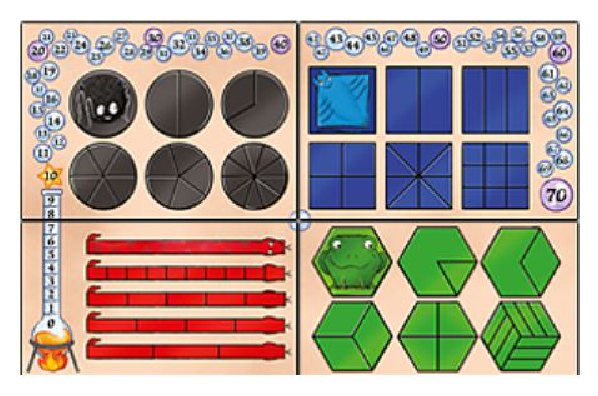
\includegraphics[width=11cm]{potions}
         \end{center}

      \partie[principes du jeu]
         Les élèves, apprentis sorciers, réalisent des potions en sélectionnant la bonne fraction d’ingrédient parmi ceux à leur disposition. Les cartes, ordonnées suivant un ordre croissant de difficulté, permettent de travailler les notions suivantes :
         \begin{itemize}
            \item représentation de fractions ;
            \item fractions supérieures à 1 ;
            \item équivalence de fraction ;
            \item somme de fractions ;
            \item décomposition de fractions, etc.
         \end{itemize}
         \begin{center}
            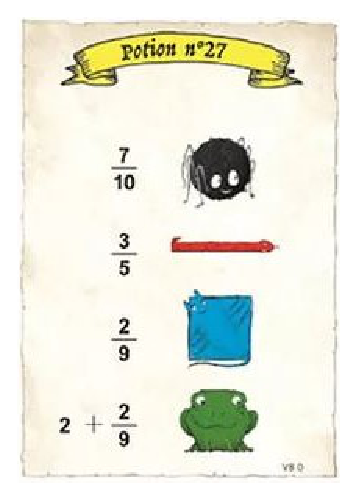
\includegraphics[width=4cm]{carte}
         \end{center}

\begin{flushright}
   \href{https://www.atelier-potions.fr}{{\small https://www.atelier-potions.fr}}
\end{flushright}
